\section{Background estimation}
\label{sec:backgroundEstimation}

Background contributions to the analysis are distinguished between reducible and irreducible backgrounds.

Reducible backgrounds arise from the misidentification of ``non-prompt'' leptons or hadrons as ``prompt'' electrons or muons,
from the misidentification of jets as $\tauh$, and from photon conversions.
We refer to ``non-prompt'' leptons as those produced in bottom or charm quark decays 
and to ``prompt'' leptons as those electrons and muons originating from decays of $\PW$ bosons, $\PZ$ bosons, or $\PGt$ leptons.
In the $\twoLeptonssZeroTau$ channel, a third source of reducible background arises from the mismeasurement of the lepton charge.
Background contributions arising from the misidentification of leptons or $\tauh$ and the background arising, in the $\twoLeptonssZeroTau$ channel, 
from the mismeasurement of the lepton charge are determined from data.
The former is referred to as the ``fakes'' and the latter as the ``flips'' background.
The estimation of these background is detailed in Sections~\ref{sec:backgroundEstimation_fakes} and~\ref{sec:backgroundEstimation_flips}, respectively.
The background arising from photon conversions is modeled using the MC simulation.
The accuracy of the modelling of this background has been validated in data~\cite{Sirunyan:2020icl}.

The main contribution to the irreducible background arises from diboson production;
from $\PZ\PZ$ production in the \zeroLeptonFourTau, \oneLeptonThreeTau, \twoLeptonTwoTau, \threeLeptonOneTau, and \fourLeptonZeroTau channels
and from $\PW\PZ$ production in the \twoLeptonssZeroTau and \threeLeptonZeroTau channels.
The production of single SM $\PHiggs$ bosons in association with $\PW$ or $\PZ$ bosons ($\V\PHiggs$), with single top quarks ($\tH$) and with top quark pairs ($\ttH$),
and the production of $\PW$ and $\PZ$ bosons in association with single top quarks ($\tV$) and top quark pairs ($\ttV$) constitute subdominant additional backgrounds.
Background events containing $\PZ$ bosons may pass the $\PZ$-veto, which is applied in all channels except the \zeroLeptonFourTau channel,
in case either one of the leptons produced in the $\PZ$ boson decay fails to get reconstructed or if the $\PZ$ boson decays to $\PGt$ leptons.
The $\tZ$ and $\ttZ$ backgrounds also include contributions from off-shell $\Ptop\APtop\Pggx$ and $\Ptop\Pggx$ production.
The background contributions arising from the associated production of $\PW$, $\PZ$, and $\PHiggs$ bosons with either single top quarks or top quark pairs
are suppressed by the $\Pbottom$-jet veto described in Section~\ref{sec:eventSelection}, but are still sizable compared to the expected $\PHiggs\PHiggs$ signal.
The irreducible backgrounds are modeled using the MC simulation.

The modelling of the dominant irreducible $\PW\PZ$ and $\PZ\PZ$ backgrounds is validated in dedicated control regions (CR),
to which we refer to as the ``\threeLeptonCR'' and ``\fourLeptonCR''.
They are based on the signal regions (SR) of the \threeLeptonZeroTau and \fourLeptonZeroTau channels,
the sole modification being that the $\PZ$-veto is inverted.
The \threeLeptonCR and \fourLeptonCR are included in the ML fit that is used to extract the $\PHiggs\PHiggs$ signal,
thereby providing in-situ constraints on the $\PW\PZ$ and $\PZ\PZ$ backgrounds.
Distributions in kinematic observables in the \threeLeptonCR and \fourLeptonCR are shown in Fig.~\ref{fig:postfitPlotsCR}.
The transverse mass, 
$\mT = \sqrt{2 \pt^{\Plepton} \ptmiss \left( 1 - \cos\Delta\phi \right)}$,
in the \threeLeptonCR is computed using the lepton that is not identified as originating from the $\PZ$-boson decay.
The symbol $\Delta\phi$ refers to the angle in the transverse plane between the momentum of this lepton and the $\ptvecmiss$ vector.
The observable $m_{4\Plepton}$ refers to the mass of the $4$-lepton system in the \fourLeptonCR.

\begin{figure}
   \centering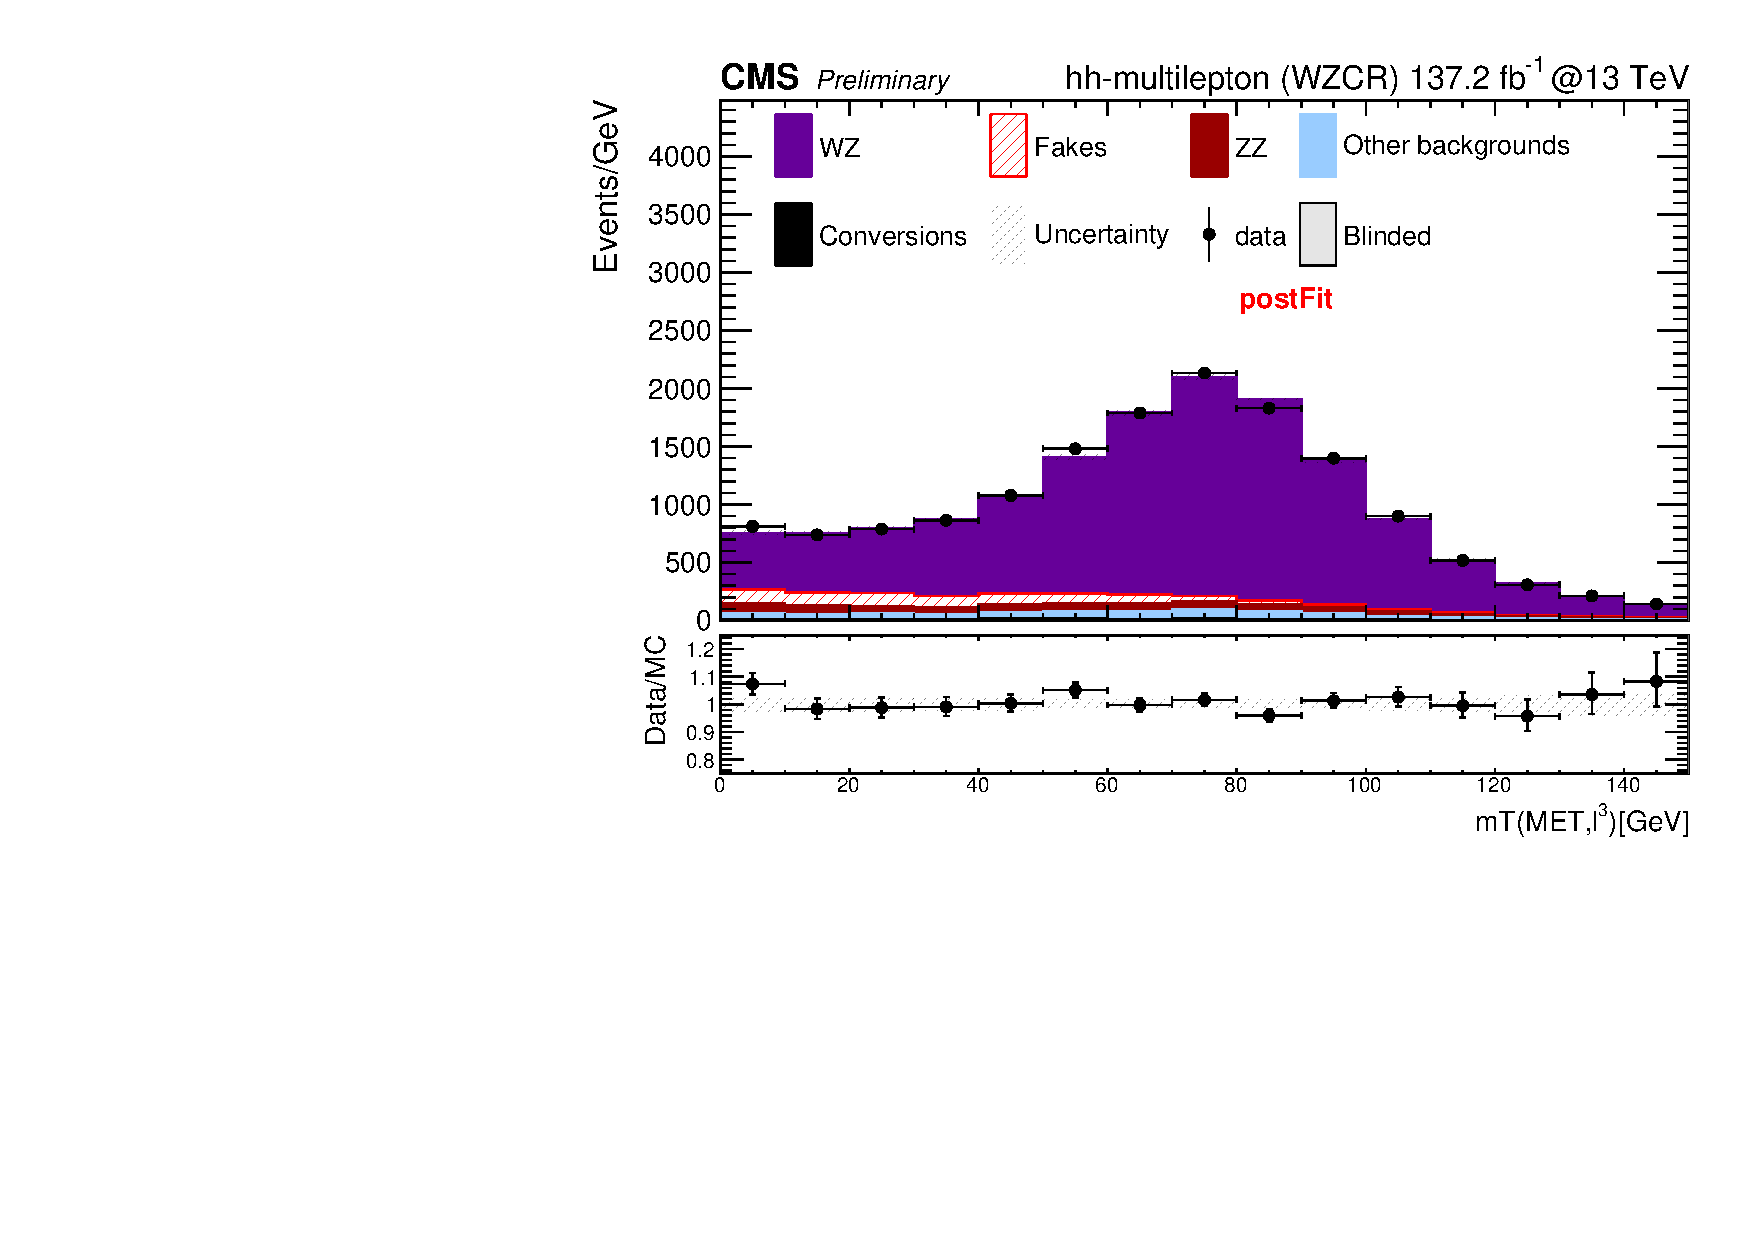
\includegraphics[width=\cmsFigWidth]{figures/postFitPlots/WZ.pdf}
   \centering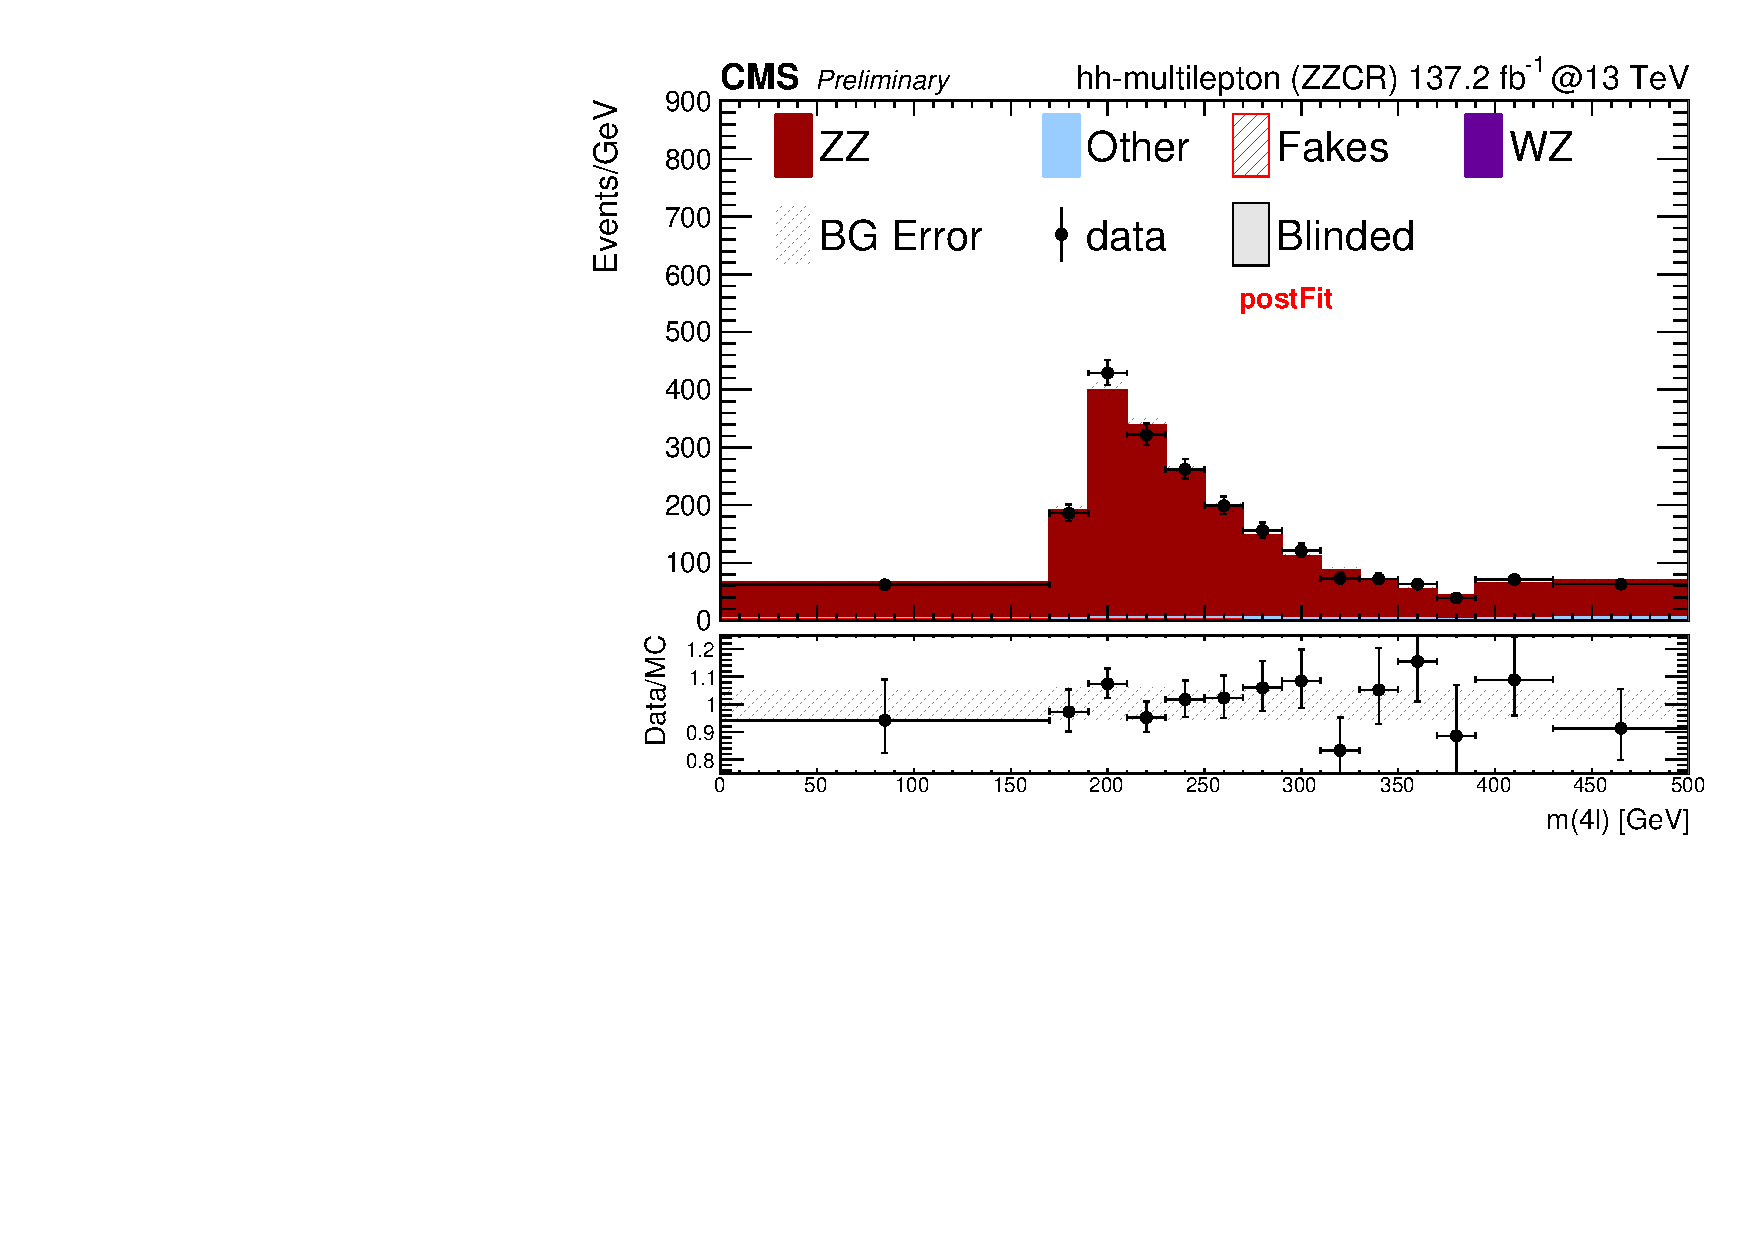
\includegraphics[width=\cmsFigWidth]{figures/postFitPlots/ZZ.pdf}
  \caption{
    Distribution in the observable $\mT$ in the \threeLeptonCR (left) and in the observable $m_{4\Plepton}$ in the \fourLeptonCR (right).
    The distributions expected for the $\PW\PZ$ and $\PZ\PZ$ as well as for other background processes
    are shown for the values of nuisance parameters obtained from the ML fit described in Section~\ref{sec:results}.
  }
  \label{fig:postfitPlotsCR}
\end{figure}

Overlap between irreducible and reducible backgrounds and between the different types of reducible backgrounds,
which would cause the double-counting of background contributions,
is avoided by categorizing each simulated event as either irreducible background or as fakes, flip, or conversion background.
The different types, or classes, of backgrounds are made mutually exclusive by ranking them in priority and assigning each simulated event to the class of highest priority for which it qualifies.
The ranking, in order to decreasing priority, is: fakes, flip, conversion, and irreducible background.
Thus, a simulated event selected in the \threeLeptonOneTau search category, which contains a reconstructed $\tauh$ that is due to the misidentification of a jet,
a reconstructed electron that is due to a photon conversion, and two genuine prompt leptons is categorized as fakes background, for example.
The evaluation of the category is based on matching reconstructed $\Pe$, $\PGm$, and $\tauh$ to their MC truth.
Electrons and muons that are misidentified as $\tauh$ and $\tauh$ that are misidentified as $\Pe$ or $\PGm$ are treated as non-fakes.


\subsection{Estimation of the ``fakes'' background}
\label{sec:backgroundEstimation_fakes}

The background from misidentified leptons and $\tauh$ is estimated using the fake-factor (FF) method~\cite{Sirunyan:2018shy}.
An estimate for the fake background contribution in the SR of each search category is obtained
by selecting a sample of events that satisfy all selection criteria of the SR for the respective search category,
except that the $\Pe$, $\PGm$, and $\tauh$ are required to pass the loose selections instead of the tight ones.
The sample of events thus obtained is referred to as the application region (AR) of the FF method.
Overlap between AR and SR is avoided by excluding from the AR those events in which all leptons and $\tauh$ satisfy the tight selections.

The estimate for the fake background contribution in the SR is obtained by applying suitably chosen weights to the events selected in the AR.
The weights, denoted by the symbol $w$, are given by the expression:
\begin{equation}
w = (-1)^{n+1} \, \prod_{i=1}^{n} \, \frac{f_{i}}{1 - f_{i}}\,
\label{eq:FF_weights}
\end{equation}
where the product extends over all $\Pe$, $\PGm$, and $\tauh$
that pass the loose, but fail the tight selection criteria,
and $n$ refers to the total number of such leptons and $\tauh$.
The symbol $f_{i}$ corresponds to the probability for an $\Pe$, $\PGm$, or $\tauh$ that passes the loose selection to also pass the tight one.
The contributions of irreducible backgrounds to the AR are subtracted based on the MC expectation of such contributions.

The probabilities $f_{i}$ for leptons are measured in multijet events, separately for electrons and muons, as described in Ref.~\cite{Sirunyan:2020icl},
and are parametrized by \pt and $\eta$ of the lepton candidate.

The $f_{i}$ for $\tauh$ are measured using $\Zmm$+jets events.
The events are selected by requiring the presence of two muons of opposite charge and mass $60 < m_{\Pgm\Pgm} < 120\GeV$,
passing the tight muon selection.
The leading and subleading muons are required to pass $\pt$ cuts of $25$ and $15\GeV$.
The events are further required to contain at least one $\tauh$ candidate that passes the loose $\tauh$ selection.
Events containing either one jet that passes the tight $\Pbottom$-tagging WP or two jets that pass the loose WP are vetoed to remove $\ttbar$ background.
The event sample thus selected is referred to as the measurement region (MR) of the FF method.
The measured probabilities $f_{i}$ for $\tauh$ are parametrized by \pt and $\eta$ of the $\tauh$ candidate.


\subsection{Estimation of the ``flips'' background}
\label{sec:backgroundEstimation_flips}

The flips background in the $\twoLeptonssZeroTau$ channel is estimated using the method described in Ref.~\cite{Sirunyan:2020icl}.
The procedure for estimating the flips background is similar to that for estimating the fakes background.
A sample of events passing all selection criteria of the SR of the $\twoLeptonssZeroTau$ channel, 
except that both leptons are required to be of OS instead of SS charge, 
are selected and assigned appropriately chosen weights.
The latter are given by the sum of the probabilities for the charge of either lepton to be mismeasured.
The probability for the charge of electrons to be mismeasured, referred to as the electron charge misidentification rate,
is determined using $\Zee$ events.
The probability for mismeasuring the charge of muons is negligible~\cite{Sirunyan:2020icl}.
